\subsubsection{Incremento 6}
\textit{\textbf{Periodo}: dal 2021-03-13 al 2021-03-18}

\myparagraph{Obiettivi}
Gli obiettivi definiti per questo incremento sono i seguenti:
\begin{itemize}
\item implementazione autenticazione del sito e visualizzazione pagina del profilo;
\item incremento della documentazione, con correzione in base a segnalazioni dei committenti;
\item inizio stesura di manuali e \textit{Allegato tecnico}\ped{G}.
\end{itemize}

\myparagraph{Attività}
Per raggiungere gli obiettivi, vengono svolte le seguenti attività:
\begin{itemize}

\item \textbf{codifica e progettazione in dettaglio}:
\begin{itemize}
\item implementazione UC1 - Registrazione cliente;
\item implementazione UC2 - Visualizzazione errori di registrazione;
\item implementazione UC3 - Login;
\item implementazione UC4 - Visualizzazione errori di login;
\item implementazione UC5 - Logout;
\item implementazione UC12 - Visualizzazione dati profilo;
\item implementazione UC13 - Modifica dati profilo;
\item creazione diagrammi UML inerenti.

\end{itemize}

\item \textbf{progettazione}: individuazione dei design pattern;

\item \textbf{pianificazione}: ristrutturazione della pianificazione secondo segnalazione;

\item \textbf{ampliamento documentazione e verifiche}:
\begin{itemize}
\item ristrutturazione dell'\AdRv{2.0.0} in base alle segnalazioni;
\item aggiornamento del \PdPv{2.0.0} in base alle segnalazioni;
\item inizio stesura del \textit{\MU{}} per i casi d'uso implementati;
\item inizio stesura del \textit{\MM{}} per i casi d'uso implementati;
\item inizio stesura dell'\textit{Allegato tecnico}\ped{G} per i casi d'uso implementati;
\item incremento del \Glossariov{2.0.0};
\item rilevazione e registrazione di metriche, esiti di verifica e obiettivi di qualità;
\item aggiornamento dei rischi rilevati;
\item calcolo e registrazione del consuntivo di periodo.
\end{itemize}

\end{itemize}
\myparagraph{Diagramma di Gantt}
\begin{figure}[H]
\centering

\centerline{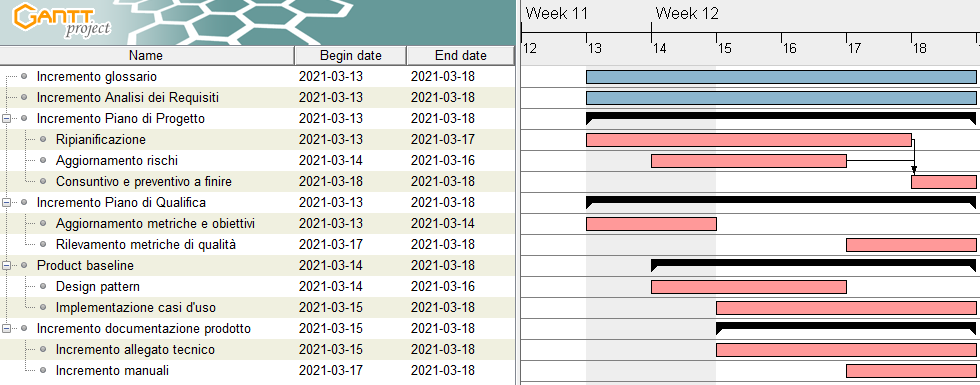
\includegraphics[scale=0.6]{res/Pianificazione/Fasi/CodificaIncrementi/ganttIncremento6}}
\caption{Diagramma di Gantt per l'incremento 6}
\end{figure}